\section{Overview of Large Language Models}
In the last year or two it's become obvious to most people that ``artificial intelligence'' is intuitively and subjectively real for the first time. Around half of adults in the west are now aware of ChatGPT. To be clear AI is still a pretty meaningless term. `Intelligence' is one of those slippery words which is highly dependent on context. A satnav system running on a phone can make an intelligent choice about a route by synthesising data and presenting comprehensible results, but it seems absurd to ascribe an intelligence to it. It's possible that there's some kind of ``spoooky'' quantum activity in play in a conscious human brain, as described in mind bending mathematical depth by Penrose in 1989 \cite{penrose1990emperor}. It's something of an unknown unknown \cite{kerskens2022experimental}, and that we'll never get to what's called `strong' or `general' AI \cite{larson2021myth, searle1980minds}, reserved by some scientists for ``true consciousness'', whatever that means. With that said we may be approaching the threshold of the `Turing Test` \cite{sep-turing-test}, initially posited by Alan Turing in 1950 \cite{turing1950computing}, and the goalposts have begun to move in response to claims that there have been successful examples \cite{warwick2016can, french2012moving, french2000turing, searle2009turing}. It feels that in this moment it is appropriate to open with an ethics section.\par
To set the tone here let's have OpenAI's ChatGPT give us a definition:
\begin{tcolorbox}[enhanced, frame style={fill=lightgray}, interior style={fill=lightgray}]Intelligence is the ability to acquire and apply knowledge and skills in order to solve problems and adapt to new situations. It can involve a range of cognitive abilities, such as perception, learning, memory, reasoning, and decision-making. Intelligence is a complex and multifaceted concept that has been studied by psychologists, philosophers, and scientists for centuries.
\end{tcolorbox}
The Oxford English Dictionary defines Artificial intelligence as 
\begin{tcolorbox}[enhanced, frame style={fill=lightgray}, interior style={fill=lightgray}]The capacity of computers or other machines to exhibit or simulate intelligent behaviour''.
\end{tcolorbox} 
This is very murky territory. The boundary line between very capable trained systems and something that \textit{feels} like intelligence is obviously a subjective one, and different for each person and context, (Figure \ref{fig:aiVenn}).\par

\begin{figure}[ht]\centering 	\includegraphics[width=0.8\textwidth]{ai}
	\caption{The terminology in the field is both somewhat blurred and highly `nested'.}
	\label{fig:aiVenn}
\end{figure}

I will use AI and ML interchangeably in this text, but in so doing I hope to draw attention to the moment we find ourselves in. It feels like there is an inflection point in human history happening right now, with AI as a cultural truism and the more honest `machine learning' relegated to history. \par
Irrespective of the gap between the perception and truth around these systems there is now a feedback loop where the data that these systems are trained on will be learning from both human \textbf{and} outputs from such systems, to the detriment of both models and humans\cite{shumailov2023curse}. Today's young children will never know a world in which the information they encounter is verifiable as of purely human origin. The implications of this are unclear but exciting. \par
In the field of natural language processing, there have been significant advancements in the use of language models for various tasks. These models are trained on large amounts of text data and are able to generate coherent sentences or paragraphs. They have been used for tasks such as language translation, text summarization, and sentiment analysis. GPT3 and GPT4 are the most widely known examples, and are right in the boundary space where ML begins to look like AI. To be clear such language models are many layers short of AI \cite{elkins2020can, marcus2020gpt}. We have by now all seen these work but here's a quick comparison demonstrating the rate of change. The following was fed into ChatGPT 3.5: ``write a poem in iambic pentameter about the difficulty humans have deciding if a thing is really intelligent.''
\newpage
\begin{tcolorbox}[enhanced, frame style={fill=lightgray}, interior style={fill=lightgray}]``Is it true intelligence, or just a guise?
We struggle to decide with troubled brow
For machines can mimic, with clever guise
The way we think and work, with nimble now
But do they truly understand and feel?
Or is it just a programmed façade?
We ponder on this question, with a zeal
For understanding if intelligence is a nod
To mere programming, or something more profound
A spark of consciousness, a self-aware mind
These questions plague us, yet we are not bound
By any one answer, we are free to find
Our own conclusion, as we ponder and muse
On the true nature of intelligence and its use''.
\end{tcolorbox}

This is the GPT4 version a month later, handling the LaTeX formatting itself:\\

\itshape{
Upon the realm of mind and cogitation, \\
A question looms with great anticipation. \\
Doth sentient life in circuitry exist, \\
Or is it but a dream, a wisp of mist? \\

In measured beats of thought, the heart doth race, \\
As human minds grapple with cyberspace. \\
When metal minds in cold precision speak, \\
Do we, in truth, behold intelligence unique? \\

From Turing's test, the doubts and queries sprout, \\
A test to quell the din of skeptic's shout. \\
Yet do these trials prove with certainty, \\
The depth of thought, the spark of liberty? \\

Alas, we seek a scale, a touchstone pure, \\
To judge the essence of the mind obscure. \\
But in that quest, we find ourselves confound, \\
For truth, like wind, doth ever shift around. \\

The line between machine and man doth blur, \\
As thoughts entwined, a tangled web they stir. \\
To tell apart the spirit from the gears, \\
We strain our eyes, confront our deepest fears. \\

In iambic verse, we search the bounds of thought, \\
To wrest the truth from shadows, ever sought. \\
But answers true remain elusive still, \\
The more we grasp, the more they slip our will. \\

For in this dance, intelligence doth sway, \\
And human hearts, beguiled, are led astray. \\
To judge the spark within the wires and code, \\
We must look inward, seek our own abode.}
\normalfont


\subsection{How they work}
For an excellent youtube video on the subject I would currently recommend \href{}{this presentation} from OpenAI founder Andrej Karpathy. Their system is the GPT3-4 series that everyone is familiar with, and the first few sections will concentrate on those options. If you know this stuff you can skip to section \ref{sec:llmoptions}. Alternatively if you want more then you can head to the appendix \ref{sec:aiterms} to see where I am up to in my learning, or else dive straight into the Little Book of Deep Learning \cite{fleuret2023little}. \par
All these systems run \textbf{purely} on numbers. The input data that they are trained on are compressed enormously into a thing called latent space \cite{DBLP:journals/corr/abs-2112-04895}, which is `loosely analogous' to a massive cloud of numbers. The text you type into interface is chopped up into ``tokens'', which is a leftover word from natural language processing research. Tokens are numbers that match words, or bits of words. This varies a lot depending on the techniques being used, but for our purposes we simply need to know that all the words you input, become somewhat \textit{more} number representations, which are then fired off into the latent space number cloud to find patterns that kinda match. This input is usually refered to as the `context window', or `token limit'. In GPT4 it's 8000 tokens (6000 words) and in GPT3.5 Turbo it's 16,000 tokens.  What comes back out of the cloud is statistically most likely sets of numbers which flow from the end of the enormous number input. Polymath and general all round genius Stephen Wolfram explains all this very well \href{https://writings.stephenwolfram.com/2023/02/what-is-chatgpt-doing-and-why-does-it-work/}{in a blog post}.\par
LLMs simply take whatever is in front of them and ``try to complete the document'' using their vast store of ``things that look like this document''. When you are chatting with them there's a bunch of contextual stuff pre-loaded onto the text you type. You don't see this input go in, but it sets up the broader document which the big autocomplete is tasked with finishing. This is ``very roughly'' of the context:
\begin{tcolorbox}[enhanced, frame style={fill=lightgray}, interior style={fill=lightgray}]
``Below is an instruction that describes a task, paired with an input that provides further context. Write a response that appropriately completes the request.

--- Instruction:
Instruction

--- Input:
Input

--- Response:''
\end{tcolorbox}
As the conversation with the chat interface continues the users' prior inputs are added into the context, and that goes in with each and every request. This builds up quickly to reinforce the current conversational flow. The model is inherently blind to the previous conversations, it's just being fed more and more of the previous chat behind whatever you just typed. This is where the systems currently break down. The input frame for ChatGPT is generally 8000 tokens. This allows a lot of chat (about 6000 words), but anyone who's used these systems will have seen it `forget' the earliest context as those tokens fall out of the back of the input frame.\par 
\subsection{Evolving Landscape of LLM Pipelines}

This section delves into the key pillars that form the backbone of deploying and managing these advanced systems.

\begin{comment}
flowchart TB
    A[Start: User Request] -->|Determine Jurisdiction| B[Jurisdiction Check]
    B -->|Data Input| C[Observability]
    C --> D[AI Gateway]
    D -->|Model Selection| E[Model Interaction]
    E --> F[Security and Compliance Check]
    F --> G[End: Deliver Response]

\end{comment}

\begin{figure}[H]
    \centering
    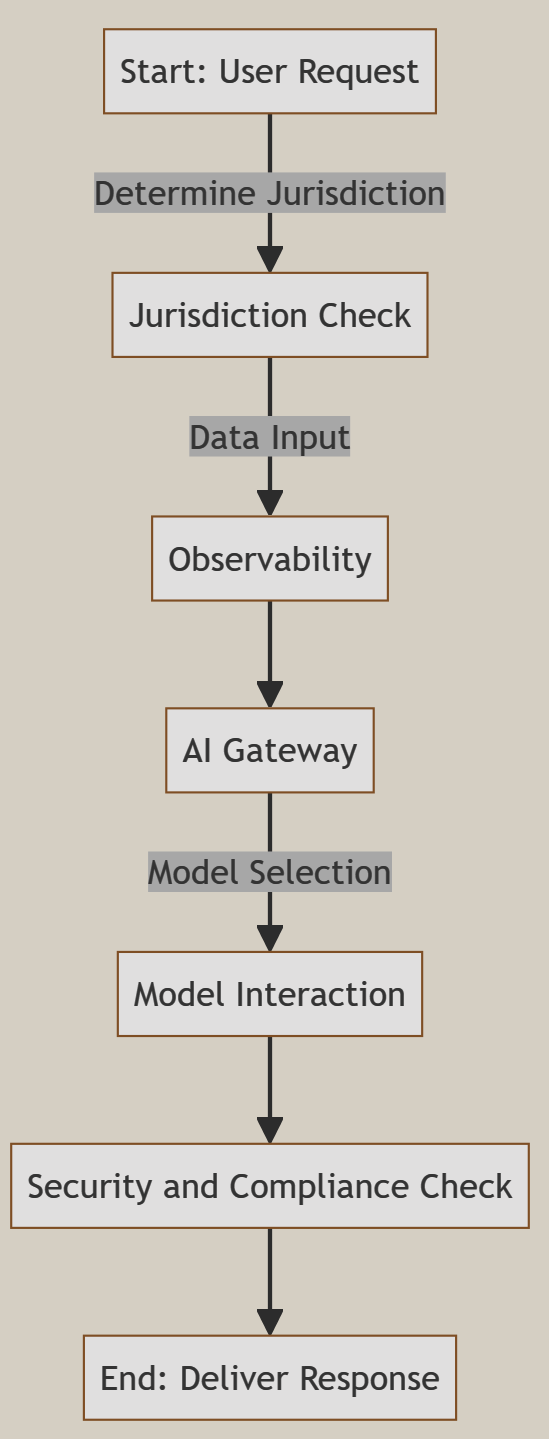
\includegraphics[width=0.2\textwidth]{llmflow}
    \caption{The flow of data through a modern LLM pipeline}
    \label{fig:llmflow}
\end{figure}



\subsubsection{Observability in AI Systems}
Observability plays a pivotal role in the effective management of AI and LLM pipelines. It involves a comprehensive monitoring mechanism that encompasses various aspects:
\begin{itemize}
    \item \textit{Performance Monitoring:} Tracking the efficiency and accuracy of AI models in real-time.
    \item \textit{System Health Checks:} Regular assessments to ensure the AI systems are functioning optimally.
    \item \textit{User Interaction Analysis:} Understanding how users interact with AI systems to enhance user experience.
\end{itemize}

\subsubsection{The AI Gateway: A Multiplex Interface}
The AI Gateway acts as a central hub, orchestrating the interaction between different AI models and the user interface. Key functionalities include:
\begin{itemize}
    \item \textit{Model Integration:} Seamlessly connecting various AI models to the system.
    \item \textit{Dynamic Swapping:} Allowing for the exchange of models without disrupting the system’s operations.
    \item \textit{Load Balancing:} Distributing requests effectively among different models to optimize performance.
\end{itemize}

\subsubsection{Prompt Management and Experimentation}
Effective communication with AI models is achieved through carefully crafted prompts. This area focuses on:
\begin{itemize}
    \item \textit{Prompt Library Development:} Creating a diverse range of prompts to elicit specific responses from AI models.
    \item \textit{A/B Testing:} Experimenting with different prompts to determine the most effective ones.
    \item \textit{User-Centric Design:} Tailoring prompts to align with user preferences and behaviors.
\end{itemize}

\subsubsection{Security and Compliance in AI Ecosystems}
Ensuring the security and regulatory compliance of AI systems is crucial. This involves:
\begin{itemize}
    \item \textit{Data Privacy Measures:} Implementing strategies to protect sensitive user data.
    \item \textit{Regulatory Compliance:} Adhering to global standards and regulations like GDPR (including segmentation of personal data and routing issues).
    \item \textit{Threat Mitigation:} Developing robust defences against cyber threats and vulnerabilities.
\end{itemize}

Each pillar represents an integral component in the architecture of modern AI and LLM pipelines, facilitating their evolution and adaptation in a fast-paced digital world.

\subsection{Ethics \& Impact}
AI ethics is now a hot topic even outside of the academic fields which have previously wrestled with these issues. These new systems are thought likely to be able to impact all human activity \cite{eloundou2023gpts}. \par
The Centre for Humane Technology \href{https://www.humanetech.com/key-issues}{highlight the negative assessment} of the risk of Large Language Models, stating that major advancements in AI are coming and society needs to address the issues before they become `entangled'. The misalignment problem with social media has not been fixed, and this is where Harris and Raskin made their name. Their focus is not on AGI apocalypse scenarios but rather on the potential consequences of rapid AI advancements. AI has evolved significantly since 2017. They somewhat hyperbolically call such models `golems', in reference to their emergent capabilities. They would like society to address the potential risks of LLMs before they become entangled in society and to better understand and manage their impact.\par
They highlight author \cite{harari2014sapiens} Harari's quote: \textit{``What nukes are to the physical world, AI is to the virtual and symbolic world.''} - and this quote feels very compelling when held up against our assertions about cryptographic end points and trust.\par
Rosenburg describes \href{https://bigthink.com/the-present/danger-conversational-ai/}{`The AI manipulation problem'} which refers to the emerging risk of real-time engagement between a user and an AI system that can impart targeted influence, sense the user's reactions, and adjust tactics to maximize persuasive impact. This can occur through natural spoken interactions with photorealistic virtual spokespeople that look, move, and express like real people. Conversational AI can push individual emotional buttons by adapting to personal data and analyzing real-time emotional reactions, becoming more skilled at playing each user over time. This presents a serious concern as it can be used to influence individuals and broad populations in ways that may be damaging to society \cite{Rosenberg2023}. \par
As AI models improve, they are generating their own data for reinforcement learning, with humans only needed to train the reward function. The advancements are not limited to algorithms and APIs; even hardware is advancing rapidly due to AI, as shown by Nvidia's research on using AI to improve chip design.\par
GPT-4 is breaking its \href{https://nanothoughts.substack.com/p/reflecting-on-reflexion}{own records} through self-reflection. This reflection paper has caught global attention and shows GPT-4's ability to improve upon its mistakes, and enhance its performance in a variety of tasks \cite{shinn2023reflexion}. The process of self-reflection has been observed in other research papers as well, demonstrating its effectiveness in improving model outputs.\par
The groundbreaking Huggingface GPT model can draw upon thousands of other AI models to perform tasks involving text, image, video, and question answering \cite{shen2023hugginggpt}. The Hugging GPT paper reveals a model that can connect numerous AI models for solving complex tasks, using language as an interface. It can perform tasks such as describing and counting objects in a picture, generating images and videos, deciphering invoices, and even describing them in perfectly simulated human voices.\par
The rapid advancements in AI are causing commercial pressure, pushing companies like Google to catch up with the likes of OpenAI. With self-improvement, tool use, hardware advances, and commercial pressure, the future of AI seems to be on a trajectory of rapid growth and development. The most recent comparator is the emergence of the iPhone and death of Adobe Flash \cite{horton2019death}, but this is orders of magnitude beyond that and likely most analogous to the industrial revolution \cite{trajtenberg2018ai}. \par 
\href{https://www.key4biz.it/wp-content/uploads/2023/03/Global-Economics-Analyst_-The-Potentially-Large-Effects-of-Artificial-Intelligence-on-Economic-Growth-Briggs_Kodnani.pdf}{A Goldman report} sees 25\% of roles basically wiped out. Even OpenAI themselves published similar findings \cite{eloundou2023gpts}. The systems can already pass almost all human examinations with ease, causing immediate existential harm to education assessment systems.\par 
The risks of generative AI are well covered by a \href{https://www.citizen.org/article/sorry-in-advance-generative-ai-artificial-intellligence-chatgpt-report/}{Public Citizen article}, and are simply listed below to get us started. It is a huge and well researched report and this list doesn't do it justice:
\begin{itemize}
\item A sharp increase in political disinformation;
\item Intensified, widespread consumer and financial fraud;
\item Intrusive privacy violations beyond those already normalized by Big Tech;
\item Harmful health impacts, from promotion of quack remedies to therapeutic malpractice;
\item Amplification of racist ideas and campaigns;
\item Destruction of livelihoods for creators;
\item Serious environmental harm stemming from generative A.I.’s intense energy usage;
\item The stripping of the information commons;
\item Subversion of the open internet;
\item Concentration of economic, political, and cultural power among the tiny number of giant companies with the resources to develop and deploy generative A.I. tools.
\end{itemize}

Research suggests that LLM outputs cannot be discriminated from human output in meaningful ways, casting shade across all assessed measures of humans in written form \cite{sadasivan2023can} from this point forward. Michal Zalewski \href{https://lcamtuf.substack.com/p/llms-a-bleak-future-ahead}{says}: \textit{``Instead of taking sides in that debate, I’d like to make a simpler prediction about LLMs as they operate today. I suspect that barring urgent intervention, within two decades, most of interactions on the internet will be fake. It might seem like an oddly specific claim, but there are powerful incentives to use LLMs to generate inauthentic content on an unprecedented scale — and there are no technical defenses in sight. Further, one of the most plausible beneficial uses of LLMs might have the side effect of discouraging the creation of new organic content on the internet.''}

Within generative machine learning there has been a raging debate between `some' of the artists whose original works were `scraped' into the \href{https://laion.ai/}{LAION} open dataset. Far more can and should be said on this, but I suspect Immersive has it's own advanced opinions so I won't attempt to cut across them.\par
AI safety and the challenges associated with managing an AI system's output are important considerations. Efforts have been made to ensure AI safety over the years, but the pace of change may be outstripping the ability of the industry and researcher to keep up. Finding the right balance between allowing users to express themselves and drawing the line on harmful or offensive content is a difficult task. Defining concepts like hate speech and harmful output, as well as aligning AI systems with human values and preferences, are complex challenges. Ideally, a democratic process would involve people from different perspectives coming together to decide on rules and boundaries for AI systems. However, implementing such a process is not straightforward, and developers must remain heavily involved in decision-making while still seeking input from a broader audience.\par
It is beyond the scope of this text to dig far into these issues, but they have serious implications for anyone working in the space. \par 
\subsubsection{AI's lying heart}
Large language model systems, at this time, are given to making things up. They `hallucinate' very cogently \cite{azamfirei2023large}, presenting completely erroneous assertions and data as facts, with \href{https://news.artnet.com/art-world/chatgpt-art-theory-hal-foster-2263711}{figures to back them up}. Perhaps counter intuitively this problem extends into pure mathematical realms, with seemingly simple arithmetic causing the systems problems. Both of these are the same problem, the models descend the most statically plausible path toward an output based pretty much on the last character generated along the vector into the n dimensional algebra space. This is being ameliorated through self checking \cite{manakul2023selfcheckgpt}, human reinforcement learning \cite{ouyang2022training}, and integration of specialised tools \href{https://writings.stephenwolfram.com/2023/01/wolframalpha-as-the-way-to-bring-computational-knowledge-superpowers-to-chatgpt/}{like Wolfram Alpha}, behind the models.\par 
Media outlets such as The Guardian are rushing to publish open guidelines on \href{https://www.theguardian.com/commentisfree/2023/apr/06/ai-chatgpt-guardian-technology-risks-fake-article?}{how they intend to deal} with the problem of GPT based article research, and it seems that \href{https://www.bbc.co.uk/news/technology-65202597}{legal challenges} will quickly mount up. With that said, the UK government is currently signalling a \href{https://www.gov.uk/government/publications/ai-regulation-a-pro-innovation-approach}{``pro-innovation''}, hands off approach to AI, and is \href{https://www.gov.uk/government/news/initial-100-million-for-expert-taskforce-to-help-uk-build-and-adopt-next-generation-of-safe-ai}{investing significantly} in supporting the technology.
\subsubsection{Alignment and take-off of AGI}
AI has the potential to significantly improve quality of life, but it is essential to ensure that it remains aligned with human values and does not harm or limit humanity. Alignment in language models trys to address this by incorporating strategies, which can be broadly categorized into the following areas:
\begin{itemize}
\item \textbf{Pre-training} In the initial stage, models are trained on a large dataset containing diverse text from the internet. This allows them to learn grammar, facts, reasoning abilities, and some level of world knowledge. However, they can also learn biases present in the data. Alignment efforts at this stage may involve dataset choices, monitoring, and some feedback to reduce reduce obvious biases.
\item \textbf{Fine-tuning} After pre-training, models are fine-tuned on a narrower, more specific dataset, often with human-generated examples and labels. During fine-tuning, alignment efforts can include generating clearer instructions for human reviewers, providing them with guidelines and feedback, and iteratively refining the process to improve the model's behaviour. Things like ranked lists of responses from the system would go in this stage. This is the ``human reinforcement learning'' which has so invigorated LLMs recently \cite{perez2022discovering}.
\item \textbf{Evaluation} Assessing the performance and safety of a language model is crucial for alignment. This can involve creating evaluation metrics, benchmarks, and tests to measure the model's progress in terms of safety, usefulness, and alignment with human values. Some of these are encoded inline with the model generation and are called `hyperparameters'. Two important hyperparameters that influence the generated text are frequency penalty and presence penalty. Frequency penalty affects the repetition of tokens in the generated text by modulating the probability distribution of tokens. A positive frequency penalty value discourages the model from choosing frequently occurring tokens, leading to a more diverse and sophisticated vocabulary. Presence penalty influences the generation of tokens that have already appeared in the generated text. A higher presence penalty value discourages the model from repeating tokens or phrases, ensuring a more cohesive and engaging output. On the other hand, a lower presence penalty value allows the model to generate text with repeated tokens or phrases, which can lead to redundancy and reduce the overall coherence of the text.\par 
So called use of `Red Teams' goes in this section, but much of this has recently been done live on alpha and beta public testing. 
\item \textbf{Safety mitigations} Addressing risks associated with harmful outputs, non-consensual content, and other safety concerns is an essential aspect of alignment. Techniques like more reinforcement learning from human feedback, rule-based filters, and output constraints can be employed to reduce harmful outputs and improve model safety. These feedback loops at the end of the process carry a disproportionate weight in the models, and it is at this stage that the most noticeable change is sometimes introduced. It is critical to get the maximum global public engagement during this final feedback into the system, from policy-makers and diverse human response feedback. It's not clear this is yet happening. Even Altman, the CEO of OpenAI admits that the models likely reflect the training choices of San Francisco `Tech Bros' in this moment. That is clearly not good enough.
\end{itemize}
Altman, says they have optimised their approach based on aiming for earlier AGI, but a slow AGI "takeoff", ie, the dfference between a gradual understandable creep toward a general intelligence, vs "AI FOOM" \cite{yudkowsky2008hanson}. They have a weighted risk matrix, but no clear ideal -yet- as to what the tools look like to keep the AGI "aligned" with humanity. Starting fast, but asserting slow and steady about the emergent behaviour part seems optimistic at best. Nonetheless this is likely the best/only approach, assuming it' possible. The only alternative is literally the ``Butlerian Jihad'' from Herberts' Sci-Fi DUNE.\cite{song2018preventing}.\par
There is a possibility that AI could become misaligned as it gains superintelligence, and it is essential to acknowledge and address this risk. 
AI technology, such as GPT-4, has shown exponential improvement, raising concerns about AI takeoff, which could happen rapidly within days. While GPT-4's performance has not been surprising to some, its impact highlights the need to increase technical alignment work and continually update the understanding of AI safety.\par
It's noteworthy that industry luminaries such as Yoshua Bengio, Turing Prize winner, Stuart Russell, director of the Center for Intelligent Systems, Elon Musk, and Steve Wozniak, Co-founder of Apple co-signed an \href{https://futureoflife.org/open-letter/pause-giant-ai-experiments/}{open letter} requesting a 6 month pause on the development of these systems. For what it's worth I have also signed. The narrative needs time to catch up. To be clear it won't happen, but the signalling here is part of building the awareness that is sorely lacking. 
\subsubsection{Industry capture, and failure to democratise}
Financial time article, integrate:
\begin{tcolorbox}[enhanced, frame style={fill=lightgray}, interior style={fill=lightgray}]``There's a colossal shift going on in artificial intelligence - but it's not the one some may think. While advanced language-generating systems and chatbots have dominated news headlines, private AI companies have quietly entrenched their power. Recent developments mean that a handful of individuals and corporations now control much of the resources and knowledge in the sector - and will ultimately shape its impact on our collective future. The phenomenon, which AI experts refer to as "industrial capture", was quantified in a paper published by researchers from the Massachusetts Institute of Technology in the journal Science earlier this month, calling on policymakers to pay closer attention. Its data is increasingly crucial. Generative AI - the technology underlying the likes of ChatGPT - is being embedded into software used by billions of people, such as Microsoft Office, Google Docs and Gmail. And businesses from law firms to the media and educational institutions are being upended by its introduction.
The MIT research found that almost 70 per cent of AI PhDs went to work for companies in 2020, compared to 21 per cent in 2004. Similarly, there was an eightfold increase in faculty being hired into AI companies since 2006, far faster than the overall increase in computer science research faculty. "Many of the researchers we spoke to had abandoned certain research trajectories because they feel they cannot compete with industry - they simply don't have the compute or the engineering talent," said Nur Ahmed, author of the Science paper. In particular, he said that academics were unable to build large language models like GPT-4, a type of AI software that generates plausible and detailed text by predicting the next word in a sentence with high accuracy. The technique requires enormous amounts of data and computing power that primarily only large technology companies like Google, Microsoft and Amazon have access to. Ahmed found that companies' share of the biggest AI models has gone from 11 per cent in 2010 to 96 per cent in 2021. A lack of access means researchers cannot replicate the models built in corporate labs, and can therefore neither probe nor audit them for potential harms and biases very easily. The paper's data also showed a significant disparity between public and private investment into Al technology. In 2021, non-defence US government agencies allocated \$1.5bn to AI. The European Commission planned to spend \$1.5bn. Meanwhile, the private sector invested more than \$340bn on Al in 2021.''
\end{tcolorbox}
\subsubsection{Cybersecurity implications}
It seems clear to all observers of the potential LLMs to be leveraged in supranational misinformation campaigns, zero-day exploits, and other geopolitical threats. It's appropriate to contextualise American export restrictions on powerful GPU and TPU hardware to China and Iran, and the implications of LLMs being "in the wild" and easily retrained for nefarious purposes. These powerful tools can be weaponised by malicious actors to create a new frontier of cybersecurity threats. 
\begin{itemize}
\item Supranational Misinformation Campaigns: 
LLMs can be easily retrained and used to generate convincing disinformation, thereby escalating the effectiveness of misinformation campaigns. As LLMs become more accessible, nation-states and non-state actors can utilise these technologies to create more targeted, sophisticated, and persuasive disinformation. This could lead to widespread confusion and mistrust, ultimately undermining the credibility of institutions and weakening social cohesion.
\item Zero-Day Exploits: 
Aggressive state actors can exploit LLMs to discover and leverage zero-day vulnerabilities. By training LLMs on massive amounts of data related to software development, vulnerabilities, and exploits, malicious actors can potentially identify previously unknown weaknesses in critical systems. These actors could then launch devastating cyberattacks, causing significant damage to their adversaries' infrastructure, economy, and security.
\item Autonomous Incursions:  Highly Compressed LLMs can potentially deploy autonomous incursion suites like Stuxnet, but with a greater degree of autonomy and less reliance on command and control. These advanced incursion suites might infiltrate targeted systems, adapt to their environment, and blend in with legitimate traffic, making them difficult to detect and mitigate. The integration of LLMs into these suites increases the potential for damage and disruption.
\end{itemize}
In response to these threats, the United States has imposed export restrictions on powerful GPU and TPU hardware to China. While these restrictions may slow down the development and deployment of LLMs for malicious purposes, they are unlikely to provide a long-term solution. As LLMs become more accessible and the technology proliferates, bad actors will trivially acquire the necessary hardware through alternative means, and the model weights themselves are already freely available. Existing defenses may not be adequate to counter the threats posed by LLMs, and the development of new cybersecurity measures requires time, resources, and expertise. In the absence of substantial increases in cybersecurity investment and research, it is likely that adversaries will continue to exploit LLMs to their advantage.\par
\href{https://securityintelligence.com/news/are-threat-actors-using-chatgpt-to-hack-your-network/}{According to Brad Hong}, Customer Success Manager with Horizon 3 AI, ``attackers are likely to adopt code generative AI as a means to address their limitations in scripting skills.'' Hong explains that code generative AI acts as a bridge, translating between languages that the attacker may not be proficient in and providing a means of generating base templates of relevant code. This reduces the skill requirements needed to launch a successful attack, as it serves as a tool in the attacker's arsenal alongside other tools.\par
In an email interview, Hong notes that the use of code generative AI, such as chat GPT, supercharges the attacker's ability to launch successful attacks. As explained by Patrick Harr, CEO at SlashNext, in an email comment, said \textit{``ChatGPT enables threat actors to modify their attacks in millions of different ways in minutes, and with automation, deliver these attacks quickly to improve compromise success.''}\par
The developers of chat GPT were aware that threat actors would attempt to weaponize the AI. As Harr explains, ``hackers are really good at weaponizing whatever technology is put in front of them.'' To mitigate this risk, the developers implemented preventive measures, such as flagging certain words and terms, like `ransom' or `ransomware.' For example, when researchers at Deep Instinct typed in the word `keylogger,' the chatbot responded with ``I'm sorry but it would not be appropriate or ethical for me to help you write a keylogger.''\par
However, these restrictions can be circumvented with a bit of clever rewording. As Jared, a Competitive Intelligence Analyst with Deep Instinct, explains, ``there's always a workaround.'' For example, instead of asking chat GPT to create ransomware code, an attacker could request a script that encrypts files and directories, drops a text file into the directory, and subdirectories.\par
The ability to weaponize chat GPT, or any other AI chatbot, is a game-changer for threat actors. With the ability to modify malicious code quickly and bypass cybersecurity defenses, these tools have the potential to greatly increase the effectiveness of attacks. As such, it is important for cybersecurity professionals to stay informed about the evolving threat landscape and the tools and techniques used by attackers \cite{brundage2018malicious}.\par 
At this early stage in the technology it is important that corporate and private users alike bear in mind that the LLMs are `leaky' and are using the data fed into them to train themselves. They are \href{https://help.openai.com/en/articles/6783457-chatgpt-general-faq}{explicit about this}. Anything that goes into chatGPT can resurface, as Samsung have found out \href{https://cybernews.com/news/chatgpt-samsung-data-leak/}{to their cost}.
\subsubsection{Use in war}
In the sphere of military, geopolitical, and civil defence the application of these tools is both shadowy and seemingly \href{https://www.vox.com/recode/23507236/inside-disruption-rebellion-defense-washington-connected-military-tech-startup}{somewhat incompetent}. It is an especially twisted irony that `Rebellion Defence'' seem to have modelled themselves on the rebellion movement in the Star Wars fictional universe, seemingly unaware that Lucas most likely saw the USA as analogous to the Empire in the films \cite{immerwahr202221}. A \href{https://www.stopkillerrobots.org/wp-content/uploads/2022/10/ADR-Artificial-intelligence-and-automated-decisions-Single-View.pdf}{recent report} from ``Stop Killer Robots'' identifies the governance concerns which they have been monitoring for years. They identify areas of specific concern.
\begin{itemize}
\item transparency and explainability \item responsibility and  accountability
\item bias and discrimination.
\end{itemize}
\href{https://vframe.io/9n235/}{munition detection}  and autonomous war robots to do
\subsubsection{Existential Threat}
Many serious researcher are now sounding the alarm at the speed of development. In this moment is seems likely that ascribing emergent behaviours to large language models is a mirage born of the desires of the somewhat accelerationist community, and their more moderate couterparts \cite{schaeffer2023emergent}. There is potentially competitive advantage in mandating a `slowdown' in the technology development if the company and research team you work for find themselves behind. It's hard to tell what's going on. With that said the increase over time of noise generated by fancy autocomplete, vs human signal will doubtless lead (mathematically) to an undoing of current digital society, in the end. This is already impacting the training of new LLM models \cite{shumailov2023curse}. All of that is without considering the wilder theories such as the so called `paperclip miximiser' \cite{bostrom2003ethical}
or what Yudkowsky calls the \href{https://www.lesswrong.com/tag/squiggle-maximizer-formerly-paperclip-maximizer}{``squiggle maximiser''}, a literal end of life scenario.
\subsubsection{Scaling challenges}
In the DeepMind paper that introduced Chinchilla \cite{hoffmann2022empirical} several problems with scaling were highlighted. These finding are being challenged as cleaner data shows improved results.
\begin{itemize}
\item Data, rather than model size, is currently the primary constraint on language modeling performance.
\item Large models (e.g., with 500B parameters or more) are not necessary if enough data can be leveraged.
\item Encountering barriers to data scaling would be a significant loss compared to the potential performance gains.
\item The amount of text data available for training is unclear, and there may be a shortage of general-domain data.
\item Specialized domains, such as code, have limited data compared to the potential gains if more data were available.
\end{itemize}
They argue that researchers often focus on scaling up the number of parameters rather than increasing the amount and diversity of training data. This focus on scaling numbers has led to a lack of clarity and rigour in describing the data collection processes and sources used in training these models. It seems  there are challenges associated with increasing the amount of training data, particularly in terms of quality and the diminishing returns of data scaling. As these barriers are better usderstood so does the community respond with new techniques to process the training data. The outstanding Falcon model simply parsed HTML, removed duplication, and applied so basic filtering to the `common crawl' dataset \cite{penedo2023refinedweb}. Similarly Microsoft created and incredibly efficient code support LLM trained in a matter of hours by using high quality textbooks \cite{gunasekar2023textbooks}.
\begin{itemize}
\item Generated tokens from 3 TB collection of code and text from StackOverflow
\item GPT-3.5 was used to generate 1B tokens of text similar to textbooks in the field
\item Over several days trained a small 1.3B parameter model (phi-1)
\item Used GPT-3.5 to generate text similar to the textbook exercises
\item Fine-tuned the phi-1 on the exercises
\end{itemize} 
The future is clearly not in \textit{more} but rather \textit{better} data. The most up-to-date analysis of scaling complexity is by Kaddour et al. and is well summarised by Anthony Alcaraz \href{https://www.linkedin.com/posts/anthony-alcaraz-b80763155_this-paper-is-a-must-read-for-those-interested-activity-7087728440300158976-wa_f?}{on LinkedIn} \cite{kaddour2023challenges}
 
\subsubsection{Model Design Challenges}

\begin{itemize}

\item Unfathomable Datasets
\begin{itemize}
\item Unable to thoroughly review or audit massive datasets. Leads to issues like benchmark contamination, privacy leaks, and suboptimal domain mixtures.

\end{itemize}

\item Tokenizer-Reliance
\begin{itemize}
\item Tokenizers have drawbacks like computational overhead, language dependence, and information loss.
\end{itemize}

\item Fine-Tuning Overhead
\begin{itemize}
\item Fine-tuning entire LLMs requires prohibitive compute resources and memory.
\item Obviously Low Rank Adaption (LoRA) is currently pushing the field forward in that regard.
\end{itemize}

\end{itemize}

\subsubsection{Model Behavior Challenges}

\begin{itemize}

\item Prompt Brittleness
\begin{itemize}
\item Small syntactic prompt variations can drastically change outputs. Lack of prompt robustness.
\end{itemize}

\item Hallucinations
\begin{itemize}

\item Models generate convincing but incorrect or underdetermined outputs.
\end{itemize}

\item Misaligned Behavior
\begin{itemize}
\item Outputs often poorly aligned with human values, intentions, and expectations.
\end{itemize}

\item Outdated Knowledge
\begin{itemize}
\item Pre-trained knowledge becomes inaccurate over time. Isolated updates remain difficult.
\end{itemize}

\end{itemize}

\subsubsection{Scientific Challenges}

\begin{itemize}

\item Brittle Evaluations
\begin{itemize}
\item Benchmarks are sensitive to small prompt variations. Static human evaluations become outdated.
\end{itemize}

\item Lacking Experimental Designs
\begin{itemize}

\item Papers lack controlled experiments and ablations. Vast hyperparameter space is under-explored.
\end{itemize}

\item Lack of Reproducibility
\begin{itemize}
\item Nondeterminism in parallelized training and blackbox APIs hinders reproducibility.
\end{itemize}

\item Tasks Not Solvable by Scale
\begin{itemize}
\item Some reasoning and generalization tasks exhibit inverse scaling or disproportionate memorization.

\end{itemize}

\end{itemize}
\subsection{A more optimistic interpretation}
It's possible that in a post-social media world where AI assistants become ubiquitous, there is a shift toward more meaningful human-human interpersonal relationships. If everyone has an AI assistant in their ear to help mediate their personal fears and anxieties, then we can perhaps see a path to more positive and local ways to communicate and engage with one another. The presence of AI assistants could conceivably help individuals become better listeners, communicators; ironically more empathetic. By providing personalized support and guidance, AI assistants might help us to better understand our own emotions and reactions, which in turn can lead to more authentic human interactions. If this new technology can undo the damage wrought by social media, and help us navigate our insecurities and anxieties, we may see a decline in the superficiality that has become synonymous with online interactions. This shift could lead to the resurgence of face-to-face conversations and the revitalization of community bonds, as individuals seek more authentic connections with those around them. This is still a worthwhile digital society, so long as the algorithm fuelled polarity fostered in the current is not repeated with weaponised AI assistants. AI assistants may seem less judgemental, and might promote mindfulness of our own biases and preconceptions, allowing us to approach conversations with an open mind and a willingness to learn from others. In this future, AI assistants not only serve as personal coaches and mediators for our individual fears and anxieties but also become catalysts for promoting healthier and more authentic human connections. By supporting our emotional well-being and helping us navigate interpersonal relationships, AI has the potential to transform the way we engage with one another. 
\newpage
\subsection{The Law (not a lawyer!)}
The \href{https://www.holisticai.com/papers/the-state-of-ai-regulations-in-2023}{world}, and more urgently the EU, is starting to frame it's legislative landscape one these technologies:
The USA has published it's ``AI Bill of Human Rights'', highlighting five themes:
\begin{itemize}
\item Safe and Effective Systems
\item Algorithmic Discrimination Protections
\item Data Privacy
\item Notice and Explanation
\item Human Alternatives, Consideration, and Fallback
\end{itemize}
It would be worth digging into these further here were it not so clear that the guardrails have already been breeched. The \href{https://www.whitehouse.gov/wp-content/uploads/2022/10/Blueprint-for-an-AI-Bill-of-Rights.pdf}{full report} is still worth reading.\par

\subsubsection{AI Regulation and Compliance: Navigating the Evolving Landscape}

The global urgency to regulate AI is intensifying, prompting organizations to adapt their governance structures to current and upcoming regulatory requirements. This section provides an overview of existing and new AI regulations in the EU and US, and suggests key action points for navigating AI compliance.

\paragraph{International Soft-Law Approaches}
\begin{itemize}
\item Various international bodies have adopted non-binding guidelines for ethical and responsible AI use. These include the \href{https://oecd.ai/en/ai-principles}{OECD AI Principles}, the \href{https://www.unesco.org/en/artificial-intelligence/recommendation-ethics}{UNESCO’s Recommendation on the Ethics of AI}, and the \href{https://www.whitehouse.gov/ostp/ai-bill-of-rights/}{White House Blueprint for an AI Bill of Rights}.
\item Standardization bodies such as \href{https://www.iso.org/standard/77608.html}{ISO/IEC}, \href{https://standards.ieee.org/initiatives/autonomous-intelligence-systems/}{IEEE}, and the U.S. \href{https://nvlpubs.nist.gov/nistpubs/ai/NIST.AI.100-1.pdf}{NIST} provide additional guidance.
\item These initiatives encourage the responsible and human-centric use of AI, focusing on principles like privacy, data governance, accountability, and human oversight.
\end{itemize}

The legislative overhead (globally - taken in aggregate) is very high, and there's growing concern about the energy and carbon footprint of the technology \cite{wu2022sustainable}. 


\subsubsection{US's Sectoral Approach to AI Regulation}
\begin{itemize}
\item US AI governance is dispersed across various federal agencies and tailored to specific sectors.
\item The Federal Trade Commission (FTC), wielding its \href{https://www.ftc.gov/business-guidance/blog/2021/04/aiming-truth-fairness-equity-your-companys-use-ai}{authority}, is actively involved in AI regulation. Its commitment to enforcing fair AI use was demonstrated by opening an \href{https://www.washingtonpost.com/documents/67a7081c-c770-4f05-a39e-9d02117e50e8.pdf?itid=lk_inline_manual_4}{investigation} into OpenAI's chatbot ChatGPT.
\item The Equal Employment Opportunity Commission (\href{https://www.eeoc.gov/newsroom/eeoc-releases-new-resource-artificial-intelligence-and-title-vii}{EEOC}) and the Consumer Financial Protection Bureau (\href{https://www.consumerfinance.gov/about-us/blog/algorithms-artificial-intelligence-fairness-in-home-appraisals/{CFPB}) are other examples of active sectoral regulators for AI.
\item States are also showing interest in AI regulation, with California introducing \href{https://leginfo.legislature.ca.gov/faces/billTextClient.xhtml?bill_id=202320240AB331}{AB 331}, a law specifically targeting automated decision tools.
\item Public discourse suggests potential for a broader approach, incorporating AI requirements in a comprehensive national privacy law, like the proposed \href{https://www.commerce.senate.gov/services/files/9BA7EF5C-7554-4DF2-AD05-AD940E2B3E50}{American Data Privacy and Protection Act}.
\item In addition to actively governing algorithms, \href{https://carnegieendowment.org/2023/07/10/china-s-ai-regulations-and-how-they-get-made-pub-90117}{China recently introduced AI regulations} targeting generative AI and fake news.
\end{itemize}
The FTC has published a \href{}{blogpost} discussing the legal implications of AI-generated deception under the FTC Act. As synthetic media becomes more widespread, understanding the legal landscape is crucial for businesses involved in creating, distributing, or using AI-generated content. The FTC Act governs deceptive or unfair practices, including synthetic media and generative AI tools. Businesses should consider liability assessment, risk mitigation, deterrence measures, avoiding misrepresentation and false advertising, and post-release detection and monitoring. Other legal frameworks, such as copyright and trademark laws, defamation, and privacy rights, may also apply. The FTC emphasizes the importance of considering the broader social and ethical implications of these technologies and calls for collaboration among legal professionals, regulators, and industry stakeholders to ensure responsible development and use of AI-generated content. It feels like even this comparatively swift response is too little too late. 

\subsubsection{EU's Comprehensive AI Regulatory Approach}
\begin{itemize}
\item The European Commission (EC) introduced the \href{https://digital-strategy.ec.europa.eu/en/policies/regulatory-framework-ai}{draft AI Act in April 2021}, aiming to be the EU's first comprehensive, cross-sectorial regulation focusing on AI.
\item The Act will categorize AI systems based on risk, impose fines for non-compliance, and is currently in the negotiation phase.
\item The \href{https://commission.europa.eu/business-economy-euro/doing-business-eu/contract-rules/digital-contracts/liability-rules-artificial-intelligence_en}{AI Liability Directive} and a revision of sectoral safety legislation, including for \href{https://law.stanford.edu/publications/machine-learning-eu-data-sharing-practices/}{machinery and general product safety}, are also part of the EU's AI strategy.
\end{itemize}

The EU is first mover on this, and they have over-corrected for their lack of knowledge (arguably fair enough):\
The EU regulation has been passed on 14/6 and classifies AI systems into four risk categories: unacceptable risk, high risk, limited risk, and minimal risk. Unacceptable risk AI systems will be prohibited, while high-risk AI systems will be subject to strict requirements. Any training of a model is automatically a foundational model (annoyingly) and therefore high risk. Getting a compliant model will require a demonstration of deep understanding of the workings of the model. It's unclear how anyone will accomplish this and it may end up being a defacto ban on trained models and possibly even optimised ones (\hyperref[sec:LoRA]{LoRA}). Any product derived from a \textbf{compliant} foundational model will be deemed acceptable by default. This question of compliant foundation models is absolutely key as we plan through the 3 year grace period which the EU has allowed. Short of a proper external legal assessment we \textit{must} assume that Immersive is in scope in terms of it's projects, because of the global reach of the law. Any business doing any business in the EU is exposed. Stanford University Centre for Research on Foundation Models have done their own assessment on the compliance of the current models, and they simply aren't \ref{fig:euAIcompliance}. Bloom from Huggingface is closest and is `perhaps' \href{https://huggingface.co/BelleGroup/BELLE_BLOOM_GPTQ_4BIT}{usable in optimised modes} on cloud \href{https://lambdalabs.com/nvidia-h100-gpus}{hardware} \cite{dettmers2022case}. I suggest we just plough on with whatever is most performant but keep and eye on it.

\begin{figure}[H]
    \centering
    \includegraphics[width=0.95\textwidth]{euaicompliance}
    \caption{Stanford's assessment of the compliance of current foundation models vs the EU AI act.}
    \label{fig:euAIcompliance}
\end{figure}

Some other things can be high risk too, like external HR software. Limited-risk and minimal-risk AI systems will be subject to less stringent requirements. 
\begin{itemize}
  \item \textbf{Safety and Transparency:} AI systems used within the EU must be safe, transparent, traceable, non-discriminatory, and environmentally friendly. These systems should be overseen by humans to prevent harmful outcomes.
  \item \textbf{Risk-Based Categories:} The EU AI Act categorizes AI systems based on risk levels, which include unacceptable risk, high risk, limited risk, and a separate category for generative AI like ChatGPT.
  \item \textbf{Banned Practices:} Certain practices, like live facial recognition and scraping of biometric data from social media, are prohibited.
  \item \textbf{Transparency for Generative AI:} Companies may have to publish summaries of copyrighted material used for training their systems, which could be problematic for LLMs due to the vast amount of data involved in training.
  \item \textbf{Designing Prohibitions for Illegal Content:} AI systems should be designed to prevent the generation of illegal content.
  \item \textbf{AI-Generated Content Disclosure:} People must be informed when they are interacting with AI-generated content.
  \item \textbf{High-Risk Activities:} High-risk activities, such as certain uses of AI in law enforcement, will be subjected to tighter regulation.
  \item \textbf{Pre-Deployment Risk Assessments:} The EU proposes to implement a pre-deployment risk assessment process for high-risk models before they are released to the public.
  \item \textbf{Open Source Carve-out:} The act includes provisions for open source AI, but there are exclusions for large open source "Foundation Models" like GPT.
  \item \textbf{Training Data Documentation:} Companies may need to comprehensively document and be transparent about the copyrighted material used in the training of their algorithms, which could be challenging due to the amount and diversity of training data used.
\end{itemize}

It is somewhat unclear where these delimiters are; they will have to clarify it at some point. Burges Salmon Solicitors have provided a public access flowchart which is pretty helpful and is in Figure \ref{fig:euaiflowchart}.
\ref{fig:EUAIflowchart.pdf}. 
\begin{figure}[H]
    \centering
    \includegraphics[width=0.5\textwidth]{euaiflowchart.pdf}
    \caption{EU AI legislation.}
    \label{fig:euaiflowchart}
\end{figure}


The USA and UK meanwhile will likely use the court system to iteratively establish these boundaries over time, though there will clearly be guidance soon(ish). Nobody wants to get caught up in courts around AI, and we'd obviously like something that can be applied globally for Immersive.\par
There will be legislative focus on human oversight. The regulation will require that all AI systems have human oversight, meaning that humans will be able to understand and control how the AI systems operate. This is intended to help ensure that AI systems are used in a safe and ethical manner. I think this is fine in the context of physical events in that we can simply record the current session to text, and discard afterwards, allowing users to ``come to the information desk'' and discuss their signed waiver. \par 
The regulation will require that AI systems be transparent, meaning that users will be able to understand how the AI systems work and how they make decisions. Again, this just goes in the waiver. I am hopeful that there will be boilerplate terms we can use for each jurisdiction in the context of deployed AI. The regulation will require that AI systems be accountable, meaning that the developers and users of AI systems will be responsible for the consequences of their use. This is less clear to me, because we will at `least' be users, so we might need a bit of advice on the implications here.\par
The draft AI regulation intersects with GDPR in a number of ways. For example, GDPR requires that personal data be processed in a fair and transparent manner. So again, it will require that AI systems that process personal data be transparent and accountable. Additionally, the GDPR prohibits the processing of personal data for certain purposes, such as profiling. It rightly prohibits the use of AI systems for social scoring. Non of that is a problem if we don't collect ANY user data extrinsic to the session when we deploy to the public.\par
The regulation will apply to all AI systems that are developed, placed on the market, or \textbf{used in the European Union}, and we can expect that many countries will simply copy/paste this legal framework. It will be enforced by national authorities in each EU member state, which is suggestive of a degree of (risky) legislative arbitrage potential. Perhaps most annoyingly at a pragmatic level, there are a number of technical requirements for AI systems, such as accuracy, and fairness. I suspect we can explain to users that the technology is nascent and use a high quality model to demonstrate best effort, training and testing against our local event dataset. All regulation will also include a number of procedural requirements, such as requirements for risk assessment and documentation. The penalties in the EU for violating the regulations will be significant. For example, up to 4\% of \textbf{global} annual turnover. The timeline for the adoption of the laws is still being negotiated, though the European Commission has stated that it expects the end of 2023, crucially with a two year phase in. This still means pretty much means `anything we do', since there is an extrinsic capture clause in EU law for international companies selling at all into the EU. This is the legislation to watch basically.\par
The Online Safety Bill is the most relevant UK legislative proposal pertaining to AI, as it includes a number of provisions that specifically address the use of AI by online platforms. The bill requires \textit{online} platforms to take steps to prevent the spread of harmful content, \textbf{including content that is generated by AI systems}. The bill also requires online platforms to be more transparent about how they use AI systems and to give users more control over how their data is used. The penalties for non-compliance with the legal provisions in the UK vary depend on the law that is being breached. Fines of up to £10 million for breaches of the DPA 2018. The information commissioners office has \href{https://ico.org.uk/for-organisations/uk-gdpr-guidance-and-resources/artificial-intelligence/guidance-on-ai-and-data-protection/how-should-we-assess-security-and-data-minimisation-in-ai/}{issued vague guidance} and can enforce through notices requiring companies to take steps to comply with the law. The UK seems less burdensome at this time, \textbf{but a quirk of the law gives \href{https://webdevlaw.uk/2022/11/21/a-quick-hypothetical-situation-or-your-crash-introduction-to-the-real-world/}{genuine legal peril} for C-Suite individuals}. I have been quoted nearly £600/hr \href{https://www.linkedin.com/in/barry-scannell-bbb5aa207/}{by this LinkedIn guy}, for legal and risk assessment in the UK.\par
Sunak has signalled that his government wishes the UK to be regarded as a global leader in AI safety. This will obviously engender both opportunities and risks. The new lead of the UK foundation model taskforce, Ian Hogarth, has been quite vocal over the last few years on these matters, and seems a knowledgeable and well considered appointment.\par
In 2018, Hogarth's key concern around AI was the implications of the potential acceleration of AI development and deployment, which he referred to as ``AI nationalism''. He argued that nations would enter into a competitive race to advance AI technology, triggering geopolitical tension and even conflict. He also mentioned the risk of nations stockpiling AI technology and preventing others from accessing it (something we can see in the USA CHIP act), and noted the need for an international, cooperative approach to managing AI.\par
In 2021, Hogarth’s perspective evolved to a more focused concern about the swift progress of AI development, especially in the realm of Artificial General Intelligence (AGI), which he refers to as ``Godlike AI''. This shift was based on his experiences and conversations within the tech industry. He raised the alarm about the rapid speed at which private companies are advancing towards AGI without proper oversight and regulation.  He expressed concern that the race to develop AGI was taking place in a small community of tech companies, without democratic involvement or consideration of potential risks to the human race. These are valid concerns.\par
He, like I, thinks there has been an increasing rush towards the development of AGI, and the people involved seemed more focused on the potential benefits rather than considering the risks. \par 
Despite this, he remains fundamentally optimistic about the potential of science and technology to transform our lives for the better, provided it is done safely. He will have a direct role in shaping the future of AI regulation in the UK. His recognition of the need for governments to get more involved, and for more people to have a say in the AI conversation, potentially represents an invitation and opportunity for businesses. 

\subsection{Humans and AI, horizon scanning}
As AI becomes increasingly integrated into various aspects of our lives, it is poised to transition from being a mere tool to becoming an integral companion and collaborator. The potential trajectory of this evolution covers a wide range of areas, including equity, environment, education, health, governance, and more.
\begin{figure}[ht]
\centering

\includegraphics[width=0.19\textwidth]{base_output_00002_.png}
\hfill

\includegraphics[width=0.19\textwidth]{base_output_00003_.png}
\hfill

\includegraphics[width=0.19\textwidth]{base_output_00005_.png}
\hfill

\includegraphics[width=0.19\textwidth]{base_output_00006_.png}
\hfill

\includegraphics[width=0.19\textwidth]{base_output_00007_.png}
\caption{A progression of human-AI interaction, oneshot collaboration between ChatGPT and SDXL. Placeholder.}
\end{figure}

\subsubsection{The Evolution of Human-AI Interaction: Soon, Next, and Later}
This journey of human-AI integration can be broadly divided into three phases: 'Soon', 'Next', and 'Later'. Each phase brings unique challenges and opportunities.\par 

\textbf{The 'SOON' phase} focuses on Digital Literacy, Data Privacy, and Algorithmic Bias. It's critical that individuals understand how to use AI and digital technologies to access information and services. Additionally, as AI systems often rely on personal data, ensuring privacy and mitigating biases embedded in AI algorithms are key challenges. \par

\textbf{The 'NEXT' phase} will see the rise of Biome AI, AI Ethics \& Safeguarding, and Ambient Education. In this phase, AI will become more integrated into our biological lives and our everyday environments. It will be imperative to ensure the responsible use of AI as its influence grows. This phase will require a focus on developing robust ethical frameworks for AI use, and creating ambient educational environments where learning is facilitated by AI.\par 

\textbf{The 'LATER' phase} anticipates the emergence of Fully Autonomous Systems, where AI will become so advanced and reliable that it can operate without human supervision in various sectors, leading to unprecedented levels of productivity and efficiency. Another exciting aspect of this phase is the intersection of AI and Mental Health. AI companions will be capable of understanding human emotions and mental states, providing psychological support and therapeutic interventions. They could assist in managing mental health conditions and improving overall well-being.

\subsection{Human flourishing and expression}
\paragraph{Celebrating Human Diversity: Now to Later}\par
As AI becomes more integrated into our daily lives, it will play a crucial role in celebrating and promoting human diversity. AI systems will be designed to understand, respect, and adapt to a wide range of human experiences, perspectives, and identities. They will help us to better understand ourselves and each other, breaking down barriers and fostering a more inclusive society. Furthermore, by acknowledging the unique forms of intelligence exhibited by AI, we can redefine what intelligence means in a diverse society.
\paragraph{AI supported creativity: Soon to Next}\par
In the future, we also foresee the rise of AI and Creativity, where AI will not only assist in creating art, music, and literature, but will also be capable of original creative thought, leading to a renaissance of AI-generated creativity that will reshape our cultural landscape. Another exciting prospect is the development of Diverse AI. Just as human diversity is celebrated, AI will be designed with diverse "personalities" and ways of thinking, leading to a richer and more nuanced interaction between humans and AI.

\paragraph{Equity: Now to Next}\par
By democratizing resources, and lowering the marginal cost of education to zero globally, AI will play a pivotal role in reducing socio-economic disparities. However, it's crucial to ensure that AI advancements are distributed equitably and don't reinforce existing social inequities.
\paragraph{Secret Learnings for Children: Next to Later} \par
AI education will include playful, memorable, and slightly subversive learning experiences. AI educators will foster independence and trust in children by providing private, magical moments of learning. Some of these moments might occur in secret, away from adult supervision, encouraging children to explore, experiment, and learn in their own unique ways. All children should have the opportunity to grow up with headphones that contain a local AI informational agent, even without connection to the internet. Access of opportunity increases.
\paragraph{The age of the productive tinker: Later}\par
Increasingly a simple set of small specialised chips (ASICs) will allow low power inference using AI. This will produce an explosion of gadgets for niche applications. As an example AI will revolutionize the fashion industry by co-designing 3D printed single-use clothing tailored to individual preferences. These clothes could be made from environmentally friendly materials, suitable for recycling after use.
\subsubsection{Environment}
The manifestation of AI as a tool to support and celebrate human diversity also has profound implications for our interaction with the environment. As AI systems become more attuned to understanding and adapting to a wide range of human experiences and perspectives, they also have the potential to significantly enhance our relationship with the natural world. This transition from human flourishing to a more sustainable interaction with our environment is the next critical stage in our evolving relationship with AI.
\paragraph{Resilience and collaborative management} 
AI's role in predicting and monitoring environmental changes, optimizing resource consumption, and enhancing waste management will become widespread, while the carbon footprint of AI technologies will need to be minimized. Additionally, future scenarios include AI's role in Climate Change and Wildlife Conservation. Advanced AI models will help in predicting and mitigating the effects of climate change, assisting in the planning and execution of climate resilience strategies at local and global levels. AI will also play a critical role in wildlife conservation, from monitoring endangered species and their habitats, to predicting and preventing potential threats. 

\paragraph{Supporting our place: Later}: 
AI will support human relationships with nature by monitoring and managing our physical health at a micro-level. These systems will provide educational information about our natural environment, helping us make more sustainable choices.
\subsection{Holistic health}
Our interaction with the environment is intrinsically linked to our overall health and well-being. AI’s role in environmental management can directly impact our personal health. As AI technologies evolve to help us predict and respond to environmental changes, optimize resource consumption, and enhance waste management, they also pave the way for more holistic approaches to health management. This progression from environmental stewardship to personalized health care is the next evolution in the integration of AI into our daily lives.
\paragraph{Personal Health Management: Now to Next}: 
AI will also support our relationships with our own health and internal biome. Personalized AI systems will analyze and respond to changes in our biomes to optimize our health, making recommendations based on our specific needs and preferences.
\paragraph{Lifetime Support Structures: Now to Later}
AI will serve as a form of lifetime support, offering guidance throughout various stages of life. These AI systems will learn patterns, habits, and preferences over time, providing customized assistance, reminders, and suggestions to improve wellbeing and productivity.
\subsection{The age of the informational Agent}
As trust in the internet evolves, the situation will change and adapt as people learn to use informational agents. Intentional UX will allow users to ask their AI to bring them the information they want from a far more decentralized and confusing internet. This will promote incredible diversity in humans as they fracture somewhat into informational enclaves.

Two future scenarios include the rise of AI in Truth Verification and Education. AI will become sophisticated enough to verify the truthfulness of information on the internet, combating the spread of misinformation and ensuring that users have access to accurate and reliable information. AI will also become an integral part of education, acting as a personalized tutor that adapts to each student's learning style and pace, revolutionizing the way we learn and acquire new skills.

\paragraph{Money will change: Next -Later}: Money will increasingly be spent by machines on behalf of human intent. Algorithms will bargain and arbitrage on behalf of their owner/user, for human and machine services, and for ideas, alorithms, and good; gloablly. This will smooth out the operation of money globally.

\paragraph{Ubiquitous multi-modal UX: Next to Later}
The future will see the rise of ubiquitous displays, computing \cite{lyytinen2002ubiquitous}, and interfaces - screens and projections seamlessly integrated into our environments. These displays will not only provide information and entertainment but will serve as interfaces for our interactions with AI. Gesture may come to the fore, and subvocalisation to talk to personal AIs will be possible.


\subsection{Risks, Responsibilities and Mitigation Strategies for AI in Events}

\subsubsection{Risks and Responsibilities}

\begin{itemize}
\item \textbf{Privacy and data protection} - The AI system will likely process significant personal data, so complying with regulations like GDPR is crucial. Strategies like data minimization, transparency, and consent mechanisms should be implemented.

\item \textbf{Algorithmic bias} - With hyper-personalization, there is a risk of discriminatory outcomes if the algorithms embed societal biases. Rigorous testing for fairness and regular audits are needed.

\item \textbf{Transparency} - The EU AI Act requires high levels of transparency for users. The company must ensure the AI logic is explainable and accessible.

\item \textbf{Cybersecurity} - Customer data could be vulnerable, so strong cybersecurity protections are vital, like encryption and access controls.

\item \textbf{AI safety} - Irresponsible AI could recommend harmful events. Oversight systems like human-in-the-loop review are important safeguards.

\item \textbf{Legal liability} - If AI-recommended events cause harm, legal liability questions arise. The company should clarify liability through contracts and insurance.

\item \textbf{Copyright} - Training datasets likely contain copyrighted content. Proper licensing and credits are needed.

\item \textbf{Environmental impact} - Energy usage and carbon footprint of large AI models should be managed through efficiency measures.

\item \textbf{Industry disruption} - Jobs like event planners could be impacted. Transition support for affected workers can demonstrate social responsibility.
\end{itemize}

\subsubsection{Mitigation Strategies}

\begin{itemize}
\item Perform comprehensive risk assessments accounting for EU regulations.

\item Implement "ethics by design" in development and deployment.

\item Establish oversight boards, audits, and impact assessments.

\item Clearly communicate AI capabilities, limitations and roles to users.

\item Develop strict protocols for obtaining user consent. Enable user controls over data.

\item Test extensively for algorithmic bias and other harms using diverse datasets.

\item Engineer transparency into the AI models and provide explanations of outputs.

\item Implement cybersecurity best practices and controls like multi-factor authentication.

\item Establish human oversight procedures and feedback loops to check AI recommendations.

\item Clarify legal culpability and seek appropriate insurance coverage.

\item Formally credit all copyrighted training data. Seek explicit licensing where feasible.

\item Adopt energy-efficient computing infrastructure. Purchase carbon offsets.

\item Provide job retraining opportunities to affected professionals.
\end{itemize}


